% !TEX program = xelatex
% Compile: xelatex slides.tex (twice)

\documentclass[aspectratio=169, 11pt]{beamer}

% ---- packages ----
\usepackage{ctex}
\usepackage{graphicx}
\usepackage{xcolor}
\usepackage{listings}
\usepackage{tikz}
\usetikzlibrary{positioning, shapes.geometric, arrows.meta, fit, calc}
\usepackage{booktabs}

% ---- theme ----
\usetheme{Madrid}
\usecolortheme{seahorse}
\setbeamertemplate{navigation symbols}{}
\setbeamertemplate{footline}[frame number]
\setbeamerfont{footline}{size=\tiny}

% Custom colors aligned with the demo's UR-cyan palette
\definecolor{urcyan}{RGB}{6, 182, 212}
\definecolor{urink}{RGB}{30, 41, 59}
\definecolor{urbody}{RGB}{248, 250, 252}

\setbeamercolor{title}{fg=urink}
\setbeamercolor{frametitle}{fg=urink, bg=urbody}
\setbeamercolor{structure}{fg=urcyan!90!black}
\setbeamercolor{block title}{bg=urcyan!15, fg=urink}
\setbeamercolor{block body}{bg=urbody, fg=urink}

% ---- listings ----
\definecolor{codekey}{rgb}{0.10, 0.30, 0.70}
\definecolor{codecmt}{rgb}{0.40, 0.55, 0.40}
\definecolor{codestr}{rgb}{0.65, 0.35, 0.10}
\lstset{
  language=Python,
  basicstyle=\ttfamily\scriptsize,
  keywordstyle=\color{codekey}\bfseries,
  commentstyle=\color{codecmt}\itshape,
  stringstyle=\color{codestr},
  showstringspaces=false,
  breaklines=true,
  frame=single,
  framerule=0.3pt,
  rulecolor=\color{black!20},
  xleftmargin=0.5em,
  tabsize=4,
}

% ---- title ----
\title[Newton VLA 课堂演示]{\textbf{基于 Newton 物理引擎与 Claude VLA \\的具身智能交互演示}}
\subtitle{答辩报告}
\author{kingcode}
\institute{}
\date{2026 年 6 月\quad\small v0.2.0}

\begin{document}

% ============================================================
\begin{frame}
\titlepage
\end{frame}

% ============================================================
\begin{frame}{目录}
\tableofcontents
\end{frame}

% ============================================================
\section{动机与目标}

\begin{frame}{为什么做这个 Demo？}
\textbf{大语言模型已经无处不在，但``身体''仍然是缺失的最后一公里。}
\vspace{6pt}
\begin{itemize}
  \item 学生很难直观感受 ``经典控制'' vs ``学习驱动'' 的分野
  \item 难以亲手验证大模型在闭环物理世界中的实际表现
  \item 大多数 VLA 教学需要 GPU 服务器或云端 API
\end{itemize}

\vspace{12pt}
\begin{block}{设计目标}
\begin{itemize}
  \item \textcolor{urcyan}{3 分钟} 课堂级现场演示
  \item \textcolor{urcyan}{零云依赖}：MacBook CPU-only
  \item \textcolor{urcyan}{60 fps} 全屏渲染
  \item \textcolor{urcyan}{毫秒级首响应}：观众输入后机械臂瞬时启动
  \item \textcolor{urcyan}{全自动回归}：所有关键路径有测试
\end{itemize}
\end{block}
\end{frame}

% ============================================================
\section{技术栈}

\begin{frame}{技术栈}
\begin{columns}[T, onlytextwidth]
\column{0.5\linewidth}
\begin{block}{物理与渲染}
\begin{itemize}
  \item NVIDIA \textbf{Newton} XPBD 物理引擎
  \item pygame 2D 草图风格渲染
  \item 闭式 3 自由度 IK
  \item Min-jerk + back-ease-out 缓动
\end{itemize}
\end{block}

\column{0.5\linewidth}
\begin{block}{人工智能与人机接口}
\begin{itemize}
  \item Claude CLI \texttt{(claude --print)} 作 VLA 大脑
  \item 关键词 + bigram LM 模糊匹配回退
  \item Google Web Speech 语音识别
  \item 中英双语关键词解析
\end{itemize}
\end{block}
\end{columns}

\vspace{12pt}
\begin{center}
\begin{tikzpicture}[every node/.style={font=\footnotesize}]
\node[draw, rounded corners=2pt, fill=urcyan!20] (n) {Newton XPBD};
\node[draw, rounded corners=2pt, fill=urcyan!20, right=8pt of n] (p) {pygame UI};
\node[draw, rounded corners=2pt, fill=urcyan!20, right=8pt of p] (c) {Claude CLI};
\node[draw, rounded corners=2pt, fill=urcyan!20, right=8pt of c] (g) {Google STT};
\node[below=4pt of $(n)!0.5!(g)$, font=\scriptsize\color{gray}] {本机 CPU，无 GPU，无云推理};
\end{tikzpicture}
\end{center}
\end{frame}

% ============================================================
\section{系统架构}

\begin{frame}{总体架构（5 层）}
\centering
\begin{tikzpicture}[
  layer/.style={
    rectangle, draw=gray!60, rounded corners=4pt,
    minimum width=8.6cm, minimum height=0.95cm,
    align=center, font=\scriptsize, fill=#1,
    inner sep=4pt,
  },
  arrow/.style={-Stealth, thick, gray!70!black},
  sidebar/.style={
    rectangle, draw=gray!60, rounded corners=4pt,
    minimum width=1.55cm, minimum height=5.6cm,
    align=center, font=\tiny, fill=yellow!25,
    inner sep=4pt, anchor=west,
  },
]
\node[layer=orange!18]                        (input)   {\textbf{输入 Input}\\
  keyboard\;\textbf{·}\;mouse\;\textbf{·}\;microphone};
\node[layer=green!15,  below=6pt of input]    (parser)  {\textbf{解析 Parser}\\
  \texttt{vla.py}\;\textbf{·}\;\texttt{voice.py}\;\textbf{·}\;\texttt{pipeline.py}};
\node[layer=cyan!15,   below=6pt of parser]   (control) {\textbf{控制 Control}\\
  \texttt{tasks.py}\;\textbf{·}\;\texttt{control.py}\;\textbf{·}\;\texttt{catcher.py}};
\node[layer=red!12,    below=6pt of control]  (physics) {\textbf{物理 Physics}\\
  \texttt{physics.py}\;\textbf{·}\;Newton XPBD};
\node[layer=purple!12, below=6pt of physics]  (render)  {\textbf{渲染 Render}\\
  \texttt{scene/}\;\textbf{·}\;\texttt{scene\_legacy.py}\;\textbf{·}\;\texttt{effects.py}\;\textbf{·}\;\texttt{sfx.py}};

\draw[arrow] (input.south)   -- (parser.north);
\draw[arrow] (parser.south)  -- (control.north);
\draw[arrow] (control.south) -- (physics.north);
\draw[arrow] (physics.south) -- (render.north);

% Fit node around all 5 layers, then place sidebar 8pt right of east edge.
\node[fit=(input)(render), inner sep=0pt] (allLayers) {};
\node[sidebar] (tel) at ([xshift=8pt]allLayers.east)
  {\textbf{telemetry.py}\\[3pt] CSV 写入\\ 每帧事件\\ 退出总结};
\foreach \src in {input, parser, control, physics, render}
  \draw[arrow, dashed, gray!60] (\src.east) -- (\src.east -| tel.west);
\end{tikzpicture}

\vspace{4pt}
\footnotesize 5 层等宽圆角块自上而下严格对齐 $\to$ 数据流单向。
Telemetry (黄) 横切监听每层关键事件。
\end{frame}

% ============================================================
\begin{frame}[fragile]{模块清单}
\centering\small
\begin{tabular}{lrl}
\toprule
模块 & 行数 & 职责 \\
\midrule
\texttt{\_\_main\_\_.py}    & 1358 & pygame 主循环、事件分发、模式切换 \\
\texttt{scene/arm.py}       &  675 & 工业风机械臂 \\
\texttt{scene\_legacy.py}   &  671 & 课堂白板渲染 \\
\texttt{physics.py}         &  659 & Newton 世界、铰接臂、\textbf{真实刚体方块} \\
\texttt{voice.py}           &  512 & 麦克风、Google STT、模糊匹配 \\
\texttt{vla.py}             &  467 & Claude CLI + 关键词回退 \\
\texttt{tasks.py}           &  429 & pick/place/stack/gesture \\
\texttt{catcher.py}         &  271 & MPC + 弹道解算 \\
\texttt{control.py}         &  214 & PD slew + NaN 拒收 \\
\texttt{experiment.py}      &  194 & \textbf{偏移塔稳定性物理课} \\
\texttt{collab.py}          &  167 & \textbf{双臂协作搭塔接力} \\
\texttt{telemetry.py}       &  163 & CSV 写入 + 公式注入防护 \\
\texttt{ik.py}              &   91 & 闭式 3-DOF IK \\
\midrule
\textbf{合计 (22 模块，实代码)} & \textbf{7653} & \footnotesize 粗体为 v0.2.0 新增/扩展 \\
\bottomrule
\end{tabular}
\end{frame}

% ============================================================
\section{三种交互模式}

\begin{frame}{交互模式 1/3：接球 MPC}
\begin{columns}[T]
\column{0.55\linewidth}
\textbf{按 \texttt{1} $\to$ 拖鼠标抛球}
\vspace{4pt}
\begin{itemize}\footnotesize
  \item 每帧实时拟合弹道：$z(t) = z_0 + v_z t - \tfrac{1}{2}g t^2$
  \item 求 $z(t) = z^\star$ 的较大正根 $\to$ 截击时刻 $t^\star$
  \item 闭式 IK 解算关节角，提交到控制器
  \item ``Commit''瞬间末端执行器画琥珀光环 (audience 看到决策点)
  \item 实战命中率 62\%--82\%
\end{itemize}
\vspace{4pt}
\textcolor{gray}{\scriptsize 判别式 $\Delta < 0$ 时退出当前预测并打一次性警告。}

\column{0.45\linewidth}
\begin{block}{为什么是\textbf{经典}控制}
\begin{itemize}\footnotesize
\item 闭式解，零优化器
\item 每帧 1\,ms 内完成
\item 弹道是高中物理，可预测
\item 对比 VLA 突出 ``学习驱动'' 的代价
\end{itemize}
\end{block}
\end{columns}
\end{frame}

% ============================================================
\begin{frame}[fragile]{交互模式 2/3：自然语言驱动 (VLA)}
\textbf{按 \texttt{2} $\to$ 输入命令 $\to$ Enter}

\vspace{6pt}
\begin{exampleblock}{Claude 把 ``pizza tower'' 解析成…}
\begin{lstlisting}[language={}, basicstyle=\ttfamily\scriptsize]
{"action":"stack", "color":null,
 "colors":["red","green","blue"],
 "target":null,
 "reason":"build a tower with default RGB"}
\end{lstlisting}
\end{exampleblock}

\vspace{4pt}
\textbf{支持的命令}
\footnotesize
\begin{itemize}
\item \texttt{pick up the red block} / \texttt{grab green} / \texttt{拿起红色}
\item \texttt{put it on the left} / \texttt{place at x=0.5}
\item \texttt{stack red green and blue} / \texttt{build a tower} / \texttt{搭个塔}
\item \texttt{drive right} / \texttt{drive to red}
\item \texttt{wave} / \texttt{say hi} / \texttt{挥手}（装饰手势）
\item \texttt{go home} / \texttt{回位}
\end{itemize}
\end{frame}

% ============================================================
\begin{frame}{核心创新：混合 VLA 解析管线}
\textbf{问题}：Claude 延迟 2--10 s，远超 60 fps 帧预算。

\vspace{4pt}
\begin{center}
\begin{tikzpicture}[
  scale=0.85,
  every node/.style={font=\scriptsize},
  event/.style={circle, fill=#1, inner sep=2pt, draw=black!40, line width=0.3pt},
  band/.style={rectangle, fill=#1, rounded corners=3pt, minimum height=12pt,
               anchor=west, inner sep=0pt, draw=black!30, line width=0.3pt},
  lane/.style={anchor=east, font=\scriptsize\itshape, color=gray!60!black},
]
% time axis
\draw[-Stealth, thick] (-0.4, 0) -- (11.5, 0) node[right] {$t$ (s)};
\foreach \x in {0, 2, 4, 6, 8, 10} {
  \draw (\x, -0.06) -- (\x, 0.06);
  \node[below=1pt] at (\x, -0.06) {\x};
}

% lane labels
\node[lane] at (-0.45, 0.7)  {input};
\node[lane] at (-0.45, 1.5)  {preflight};
\node[lane] at (-0.45, 2.3)  {Claude};
\node[lane] at (-0.45, 3.1)  {arm};

% lane 1
\node[event=blue!60] (in) at (0, 0.7) {};
\node[above right=0pt and 2pt] at (in) {\textit{输入}};

% lane 2 — preflight
\node[band=green!55, minimum width=3pt] at (0, 1.5) {};
\draw[->, semithick, green!55!black] (0.12, 1.5) -- (1.1, 1.5);
\node[right=1pt, green!45!black] at (1.1, 1.5) {\textbf{1 ms}};

% lane 3 — Claude
\node[band=orange!55, minimum width=9cm] at (0, 2.3) {};
\node[white] at (4.5, 2.3) {\bfseries Claude refining…};
\node[event=red!65] (refine) at (9, 2.3) {};
\node[above right=0pt and 2pt] at (refine) {Claude 复审 (\textbf{9.4 s})};

% lane 4 — arm
\node[band=blue!35, minimum width=10.5cm] at (0.1, 3.1) {};
\node at (5.35, 3.1) {Arm 持续动作 (pick $\to$ stack $\to$ \dots)};
\end{tikzpicture}
\end{center}

\vspace{6pt}
\begin{enumerate}\footnotesize
\item 关键词 \texttt{\_keyword\_fallback} 同步运行 ($\sim 1$\,ms) $\to$ \textbf{机械臂立刻动}
\item Claude 后台 daemon thread 跑 \texttt{claude --print}（$\sim 9$\,s）
\item Claude 返回后\textbf{比较} preflight 结果：相同$\to$静默确认，不同$\to$打日志
\item generation counter 防止旧线程结果覆盖新命令
\end{enumerate}

\textbf{效果}：观众感知的命令响应延迟从 9.4 s $\to$ 1 ms。
\end{frame}

% ============================================================
\begin{frame}{交互模式 3/3：手势装饰}
\textbf{按 \texttt{2} 输入 ``wave'' / ``dance'' / ``bow'' / ``point at the audience''}

\vspace{6pt}
\begin{columns}
\column{0.5\linewidth}
\begin{itemize}\footnotesize
  \item \texttt{make\_wave}：手臂上举 + 左右扫
  \item \texttt{make\_point}：左/右/audience 三方向
  \item \texttt{make\_bow}：前倾下俯保持后归位
  \item \texttt{make\_dance}：4 拍方框轨迹
\end{itemize}

\column{0.5\linewidth}
\begin{block}{为什么不只是抓物？}
\footnotesize
教学叙事需要``表情''
\\— 手势让机器人看起来\textbf{有意图}，
而不只是一台精确但冷漠的设备。
\end{block}
\end{columns}

\vspace{8pt}
\textbf{修过的一个 CRITICAL bug}：手势的 preflight 白名单原本
漏掉了 \texttt{wave/point/bow/dance}，导致所有手势必须等
Claude 9.4 s 才能触发。修复后\textbf{瞬时响应}。

\vspace{4pt}
\textcolor{gray}{\scriptsize \texttt{point} 的方向参数原来被
``颜色过滤''强制过滤为合法颜色，导致所有 point 都退化为 ``left''。
也修了。}
\end{frame}

% ============================================================
\section{工业模式：双臂并行}

\begin{frame}[fragile]{Arm B：固定底座工件搬运}
\begin{columns}[T]
\column{0.55\linewidth}
\textbf{\texttt{--industrial}}：第二只机械臂 Arm B 固定在右侧
支架上（FK-only，不进 Newton 物理）。
\vspace{4pt}
\begin{itemize}\footnotesize
\item 与 Arm A 共享 \texttt{world.blocks}（pick 互斥）
\item 拥有专属 ``workpiece'' 灰色方块
\item 空闲时循环搬运工件（基础行为）
\item 与 Arm A \textbf{完全并行}：你按 1 抛球时它仍在搬运
\end{itemize}
\vspace{2pt}
\footnotesize\textcolor{urcyan}{v0.2.0：空闲搬运已升级为 \texttt{--collab} 双臂协作搭塔（见后）。}

\column{0.45\linewidth}
\begin{block}{修过的一个潜在 bug}
\scriptsize
原 \texttt{\_ensure\_reachable} 给任何臂都派 \texttt{world.drive\_to(...)}，
\\— 这会把 Arm A 的底盘\textbf{拖来拖去}。
\\— 修：固定臂 (anchor 已设) 跳过 drive。
\end{block}
\end{columns}

\vspace{8pt}
\begin{lstlisting}[basicstyle=\ttfamily\scriptsize]
def _ensure_reachable(self, world_xz):
    if self.anchor_world_x is not None:
        return []  # fixed-base arm: no drive
    ...
\end{lstlisting}
\end{frame}

% ============================================================
\begin{frame}{演示截图 1/5：IDLE 工业模式}
\centering
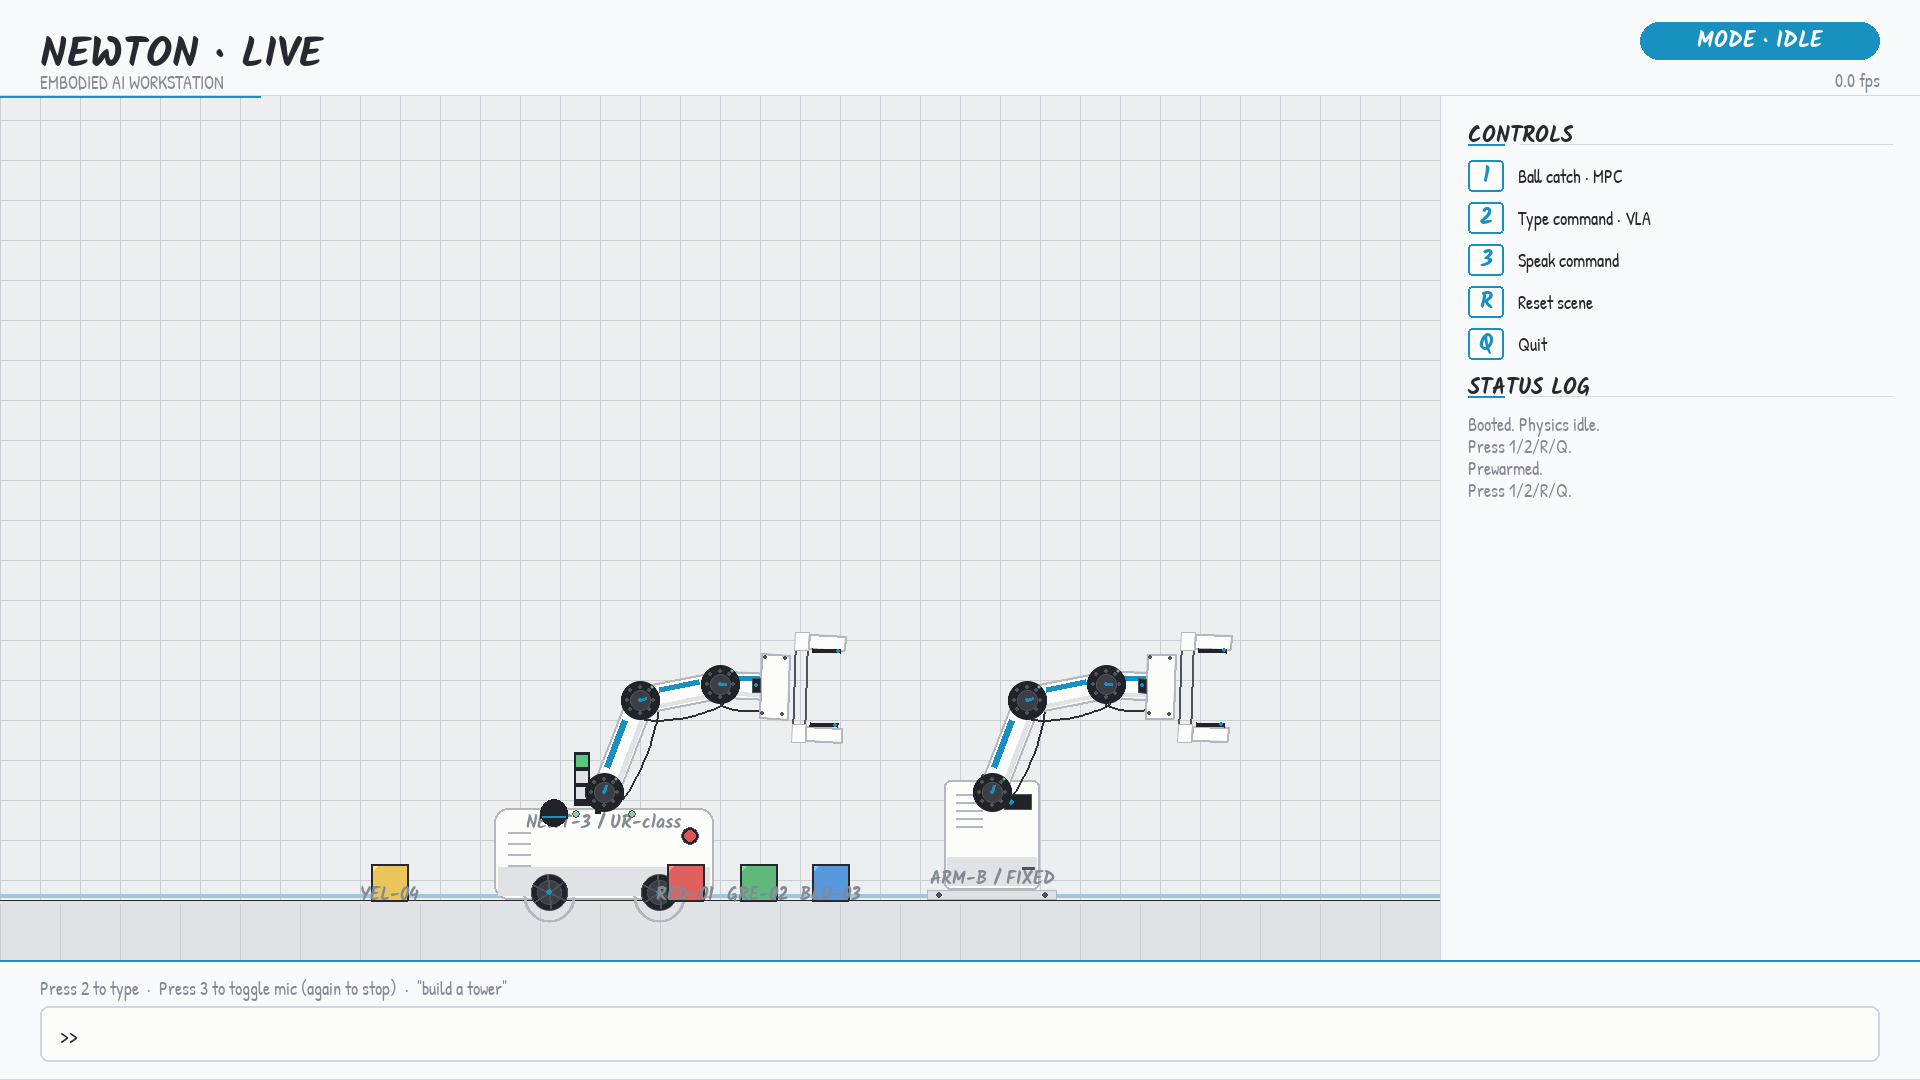
\includegraphics[width=0.85\linewidth]{figures/industrial_view.png}

\vspace{2pt}
\footnotesize 左：移动底盘 Arm A（学生命令驱动）。右：固定
Arm B 自主搬运 workpiece（基础工业模式；\texttt{--collab} 时升级为协作搭塔）。
5 个方块、控制面板、状态日志一览。
\end{frame}

% ----
\begin{frame}{演示截图 2/5：IDLE 课堂模式}
\centering
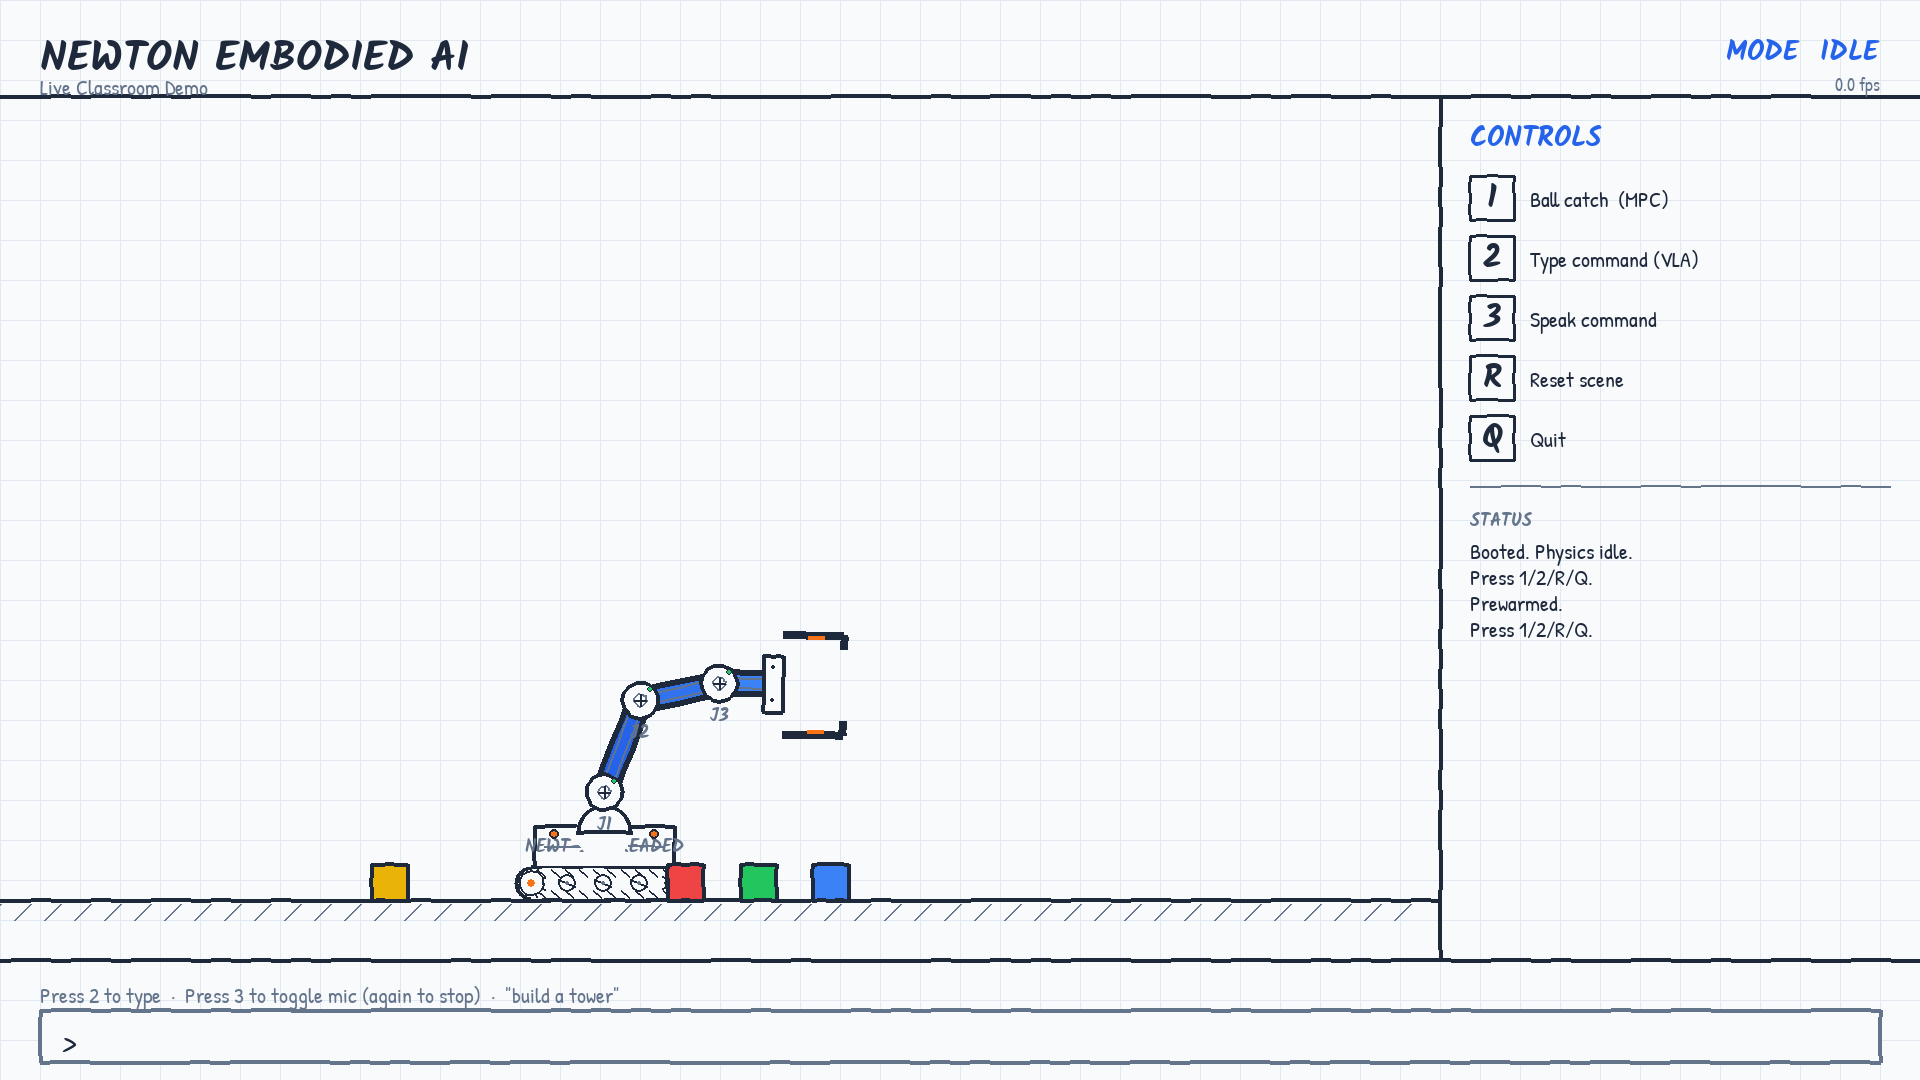
\includegraphics[width=0.85\linewidth]{figures/classroom_view.png}

\vspace{2pt}
\footnotesize 默认课堂白板风。手绘草图机械臂 + 4 教学色方块，
模拟黑板演示。无 Arm B。
\end{frame}

% ----
\begin{frame}{演示截图 3/5：BALL CATCH 实时追踪}
\centering
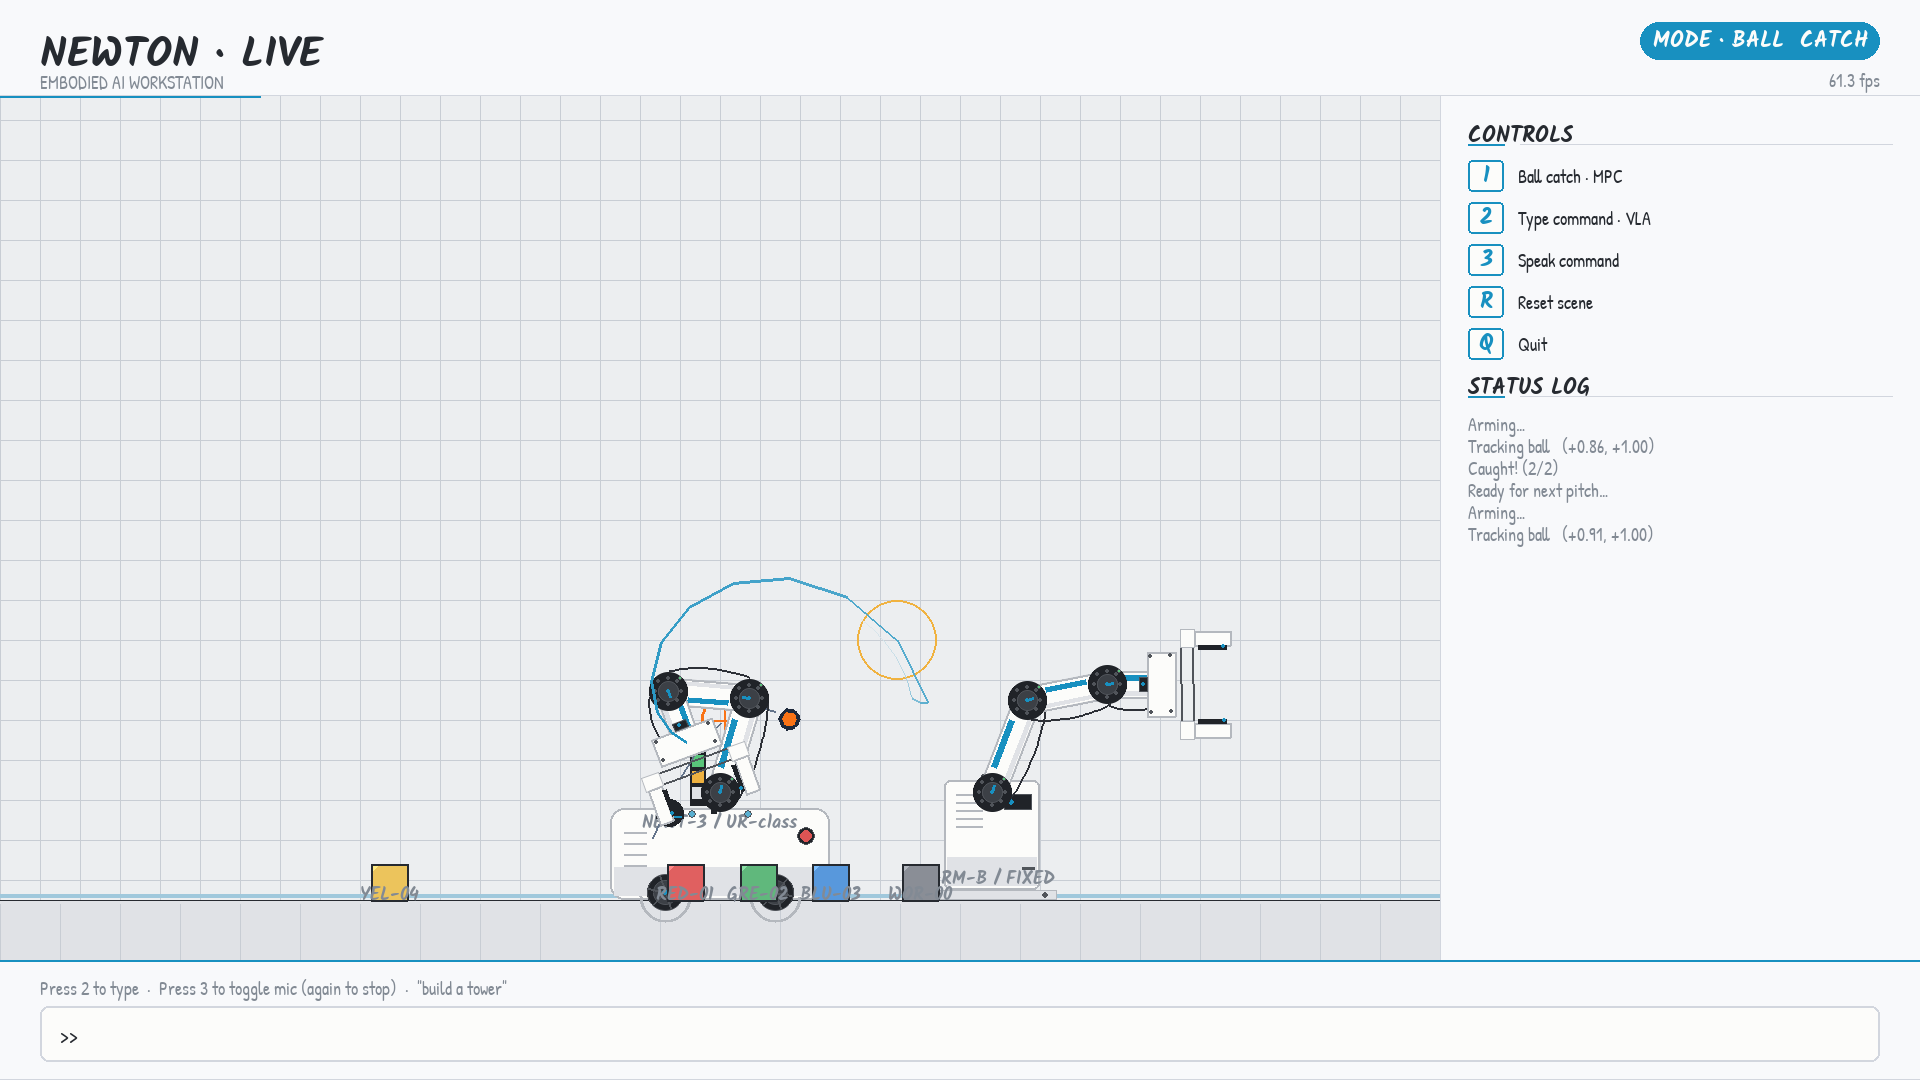
\includegraphics[width=0.85\linewidth]{figures/catch_industrial.png}

\vspace{2pt}
\footnotesize \textbf{蓝色轨迹}：每帧采样小球位置；
\textbf{橙色圆环}：\texttt{catcher.\_predict()} 计算的截击点。
状态日志显示连续 ``Caught! (2/2)''。
\end{frame}

% ----
\begin{frame}{演示截图 4/5：TASK EXEC 自主堆塔}
\centering
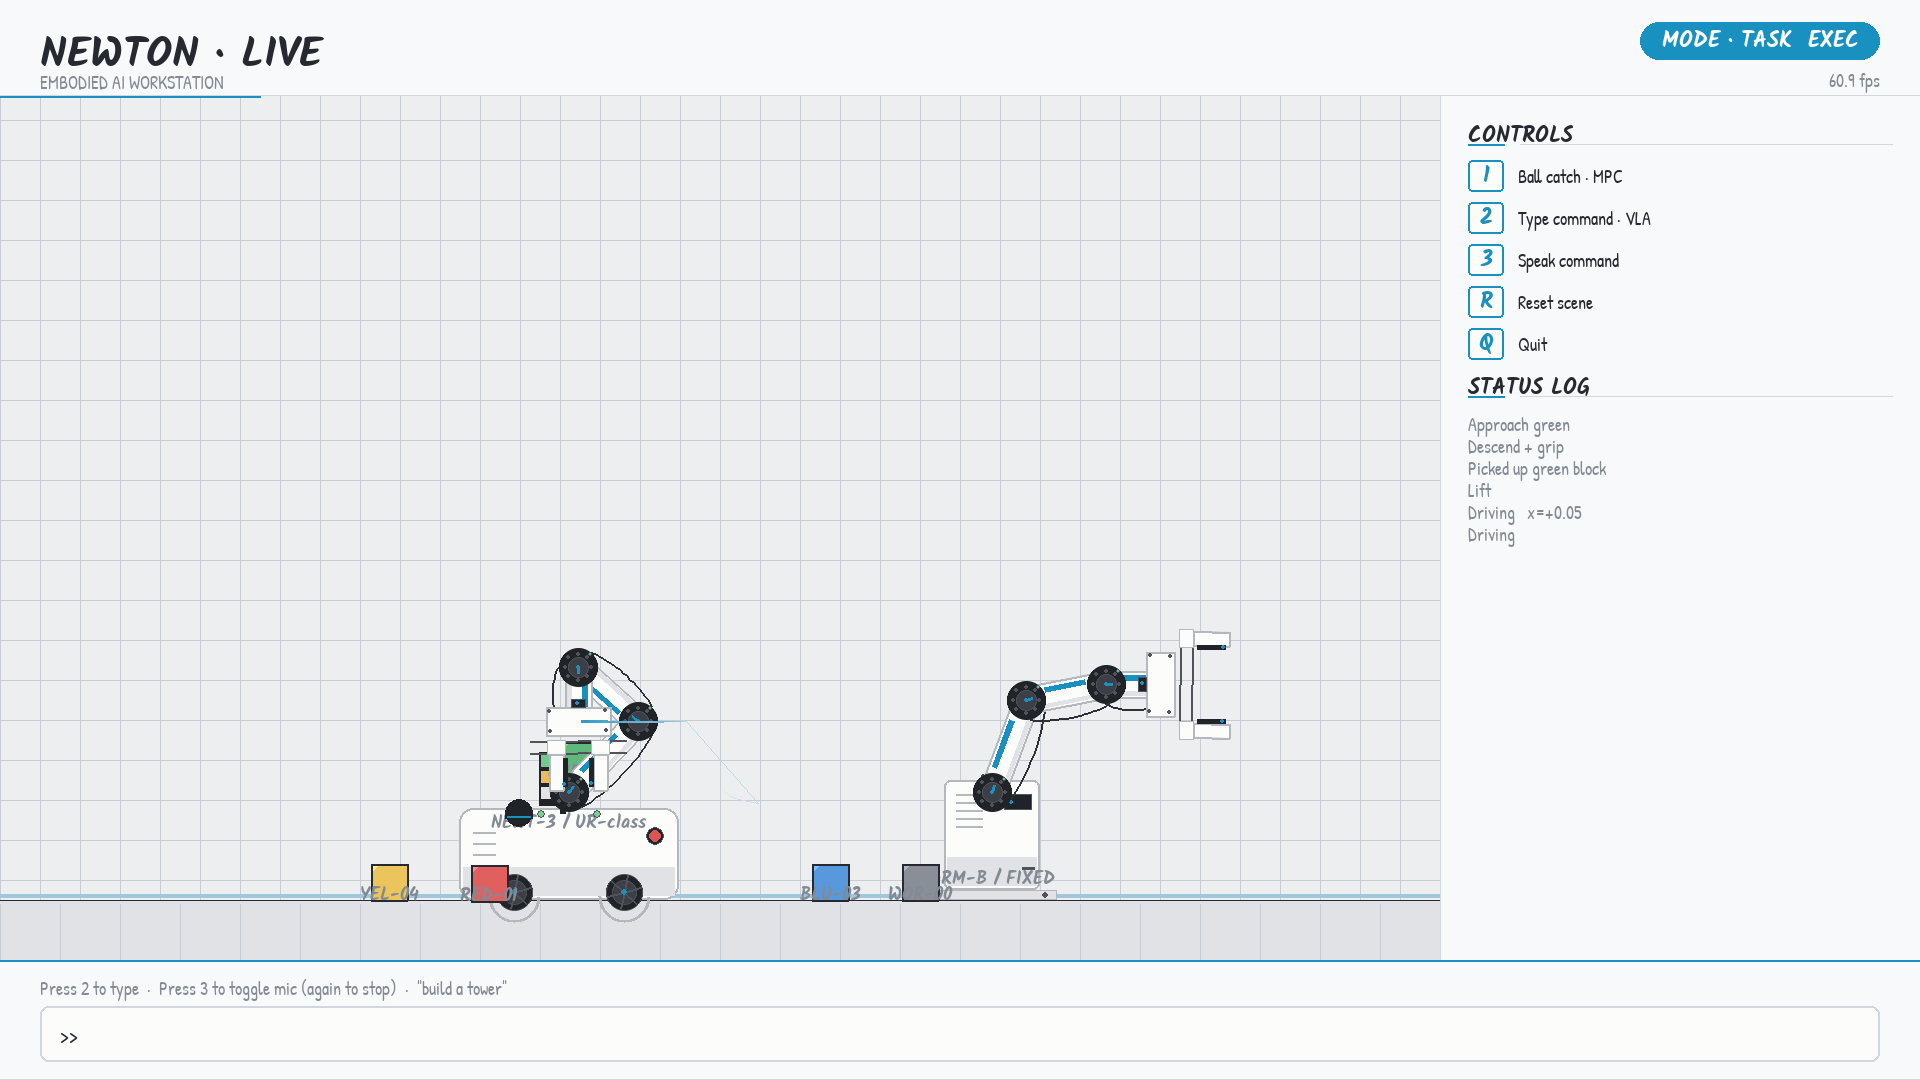
\includegraphics[width=0.85\linewidth]{figures/stack_industrial.png}

\vspace{2pt}
\footnotesize Arm A 持\textbf{绿块}向左前行，红块已就位。
status log 完整呈现 \texttt{Approach $\to$ Descend + grip
$\to$ Picked up $\to$ Lift $\to$ Driving} 五步流水。
\end{frame}

% ----
\begin{frame}{演示截图 5/5：VLA \textbf{AI · PARSED} 侧栏}
\centering

\includegraphics[width=0.9\linewidth]{figures/vla_panel_industrial.png}

\vspace{2pt}
\footnotesize 用户输入 \texttt{"build a tower of red green
and blue"} $\to$ Claude 后端 \texttt{9564 ms} 返回 $\to$
解析为 \texttt{stack [red,green,blue]}。塔已堆好红+绿，
正持蓝块行进。\textbf{Claude 在想什么观众一目了然。}
\end{frame}

% ============================================================
\section{v0.2.0：真实物理 · 双臂协作 · 物理课}

\begin{frame}[fragile]{真实刚体方块 \texttt{--real-blocks}}
\textbf{默认 teleport（Python 解析驱动）$\to$ \texttt{--real-blocks} 让方块成为真正的
Newton XPBD 刚体}：会堆叠、会碰撞、会倒塌。
\vspace{4pt}
\begin{columns}[T]
\column{0.52\linewidth}
\textbf{难点：XPBD 没有 weld / 焊接约束}\\
\footnotesize（equality 约束是 MuJoCo 求解器专属）。怎么让夹爪"抓住"方块？
\vspace{4pt}
\begin{block}{KINEMATIC $\leftrightarrow$ DYNAMIC 切换}
\footnotesize
\begin{itemize}
\item 抓住：\texttt{grab\_block} 把 body 设 \texttt{BodyFlags.KINEMATIC}，每帧把它的位姿写成夹爪 TCP（求解器原样透传）
\item 放下：设回 \texttt{DYNAMIC}，在重力下落到下方物体上
\item 切换后必须 \texttt{notify\_model\_changed} 让 XPBD 重算 kinematic 集
\end{itemize}
\end{block}

\column{0.48\linewidth}
\begin{block}{工程细节}
\footnotesize
\begin{itemize}
\item 碰撞过滤：块$\leftrightarrow$块、块$\leftrightarrow$地 \textbf{开}；臂$\leftrightarrow$块、球$\leftrightarrow$块 \textbf{关}（臂用 kinematic 抓取，物理接触只会和 PD 控制器打架）
\item \texttt{\_held\_body\_ids} 防双抓 / 防空放
\item OOB 恢复跳过手持块（避免抖动）
\item 20 cm 立方体，\texttt{iterations=8, substeps=2, relaxation=0.8}
\end{itemize}
\end{block}
\end{columns}
\end{frame}

% ----
\begin{frame}{双臂协作搭塔 \texttt{--collab}}
\textbf{舞台空闲 3 s 后自动开演}：两臂接力搭塔，是"恰好是机器人协作的屏保"。
\vspace{4pt}
\begin{columns}[T]
\column{0.55\linewidth}
\begin{block}{接力流水线 (\texttt{CollaborativeBuild})}
\footnotesize
\begin{enumerate}
\item Arm A（移动）取色块 $\to$ 放到 \textbf{交接槽} $x=1.50$
\item Arm B（固定）从交接槽取走 $\to$ 堆到塔列 $x=1.70$
\item 红$\to$绿$\to$蓝 自底向上；admire 2.5 s
\item \textbf{角色互换}拆塔（自顶向下，绝不抽承重块）
\item 归位 $\to$ 循环
\end{enumerate}
\end{block}

\column{0.45\linewidth}
\begin{block}{安全联锁}
\footnotesize
\textbf{单交接槽}就是全部互锁：A 只在槽空时投放，B 取走的瞬间释放槽。无显式碰撞几何，靠 \textbf{时序不对称}（B 抬升 $\sim$2 s vs A 补给 $\sim$10 s）保证两臂永不同时伸向槽。
\end{block}
\vspace{2pt}
\footnotesize\textcolor{urcyan}{观众一动（抛球/输入/语音）$\to$ 立即让出双臂。}
\end{columns}

\vspace{4pt}
\footnotesize\textcolor{gray}{修过的 bug：collab 曾在任何 \texttt{--bench} 下静默失效（误挂在 Arm B 的 idle 门控上）$\to$ 已给独立门控。}
\end{frame}

% ----
\begin{frame}{Arm B 物理课：偏移塔稳定性 \texttt{--experiment}}
\textbf{让真实 XPBD 当裁判}：Arm B 用 3 块灰色工件按\textbf{逐层偏移} $0\to4\to9$ cm 堆塔，
物理判定倒不倒——\textbf{判据是算出来的，不是脚本写死的}。
\vspace{6pt}
\begin{columns}[T]
\column{0.52\linewidth}
\begin{block}{倒塌判据（高中物理）}
\footnotesize
半宽 $r=10$ cm 的等质量立方体，上两层组合重心偏离底块中心 $1.5d$。
重心铅垂线越出底块支撑面即倒：
\[ 1.5\,d > r \;\Rightarrow\; d > \tfrac{r}{1.5} \approx \mathbf{6.67\ \text{cm}} \]
\scriptsize $\Rightarrow$ 4 cm 轮稳、9 cm 轮倒、0 cm 是基线。
\end{block}

\column{0.48\linewidth}
\begin{block}{实现}
\footnotesize
\begin{itemize}
\item \texttt{toppled()}：任一块 $|\text{angle}|>0.30$ rad（$\sim17°$）或顶块高度跌落 $>r$
\item 重心铅垂线 + 支撑括号实时叠加，越界翻 \textcolor{orange!80!black}{琥珀色} + ``CoM\,$\to$\,OUT''
\item 向 $-x$ 倒（散块落进空带，自动收拾）
\item 隐含 \texttt{--real-blocks + --industrial}；与 \texttt{--collab} 互斥
\end{itemize}
\end{block}
\end{columns}
\end{frame}

% ----
\begin{frame}{偏移塔实测：Stable $\to$ Stable $\to$ TOPPLED}
\centering
\begin{columns}[T]
\column{0.33\linewidth}
\centering
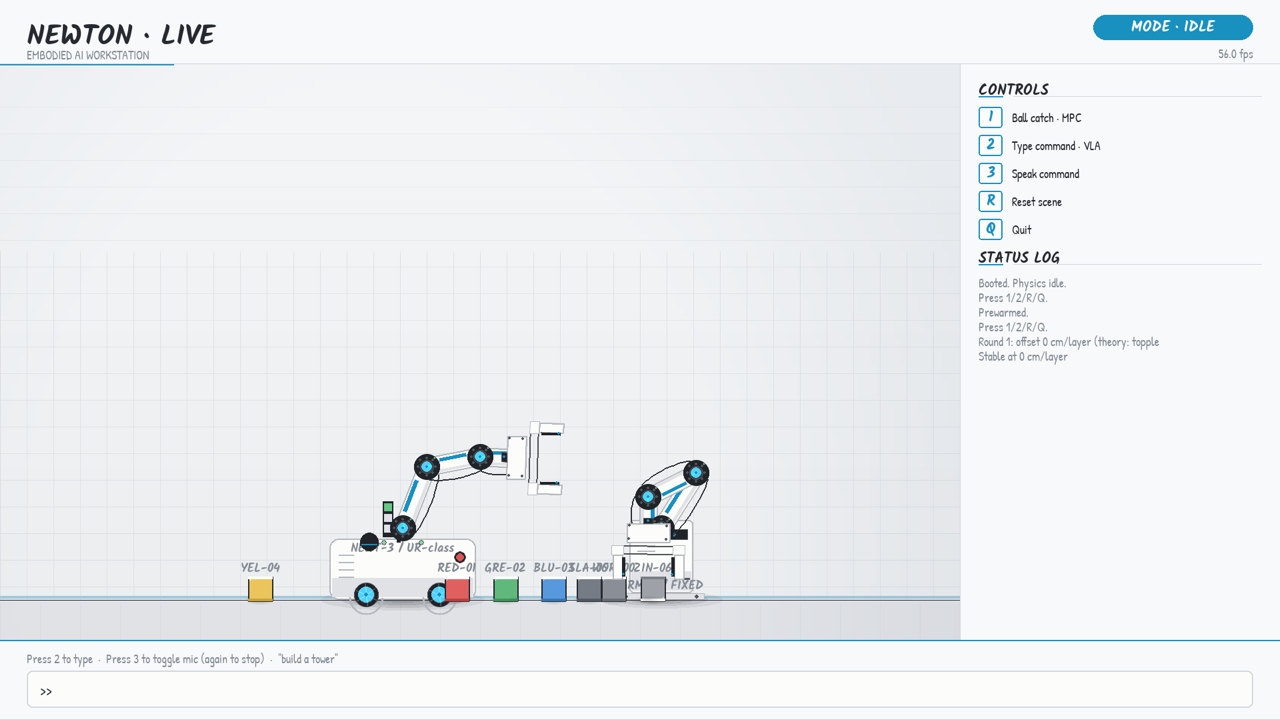
\includegraphics[width=\linewidth]{figures/experiment_aligned.png}\\
\footnotesize \textbf{0 cm} · 重心正对底座 · \textcolor{green!50!black}{稳}
\column{0.33\linewidth}
\centering
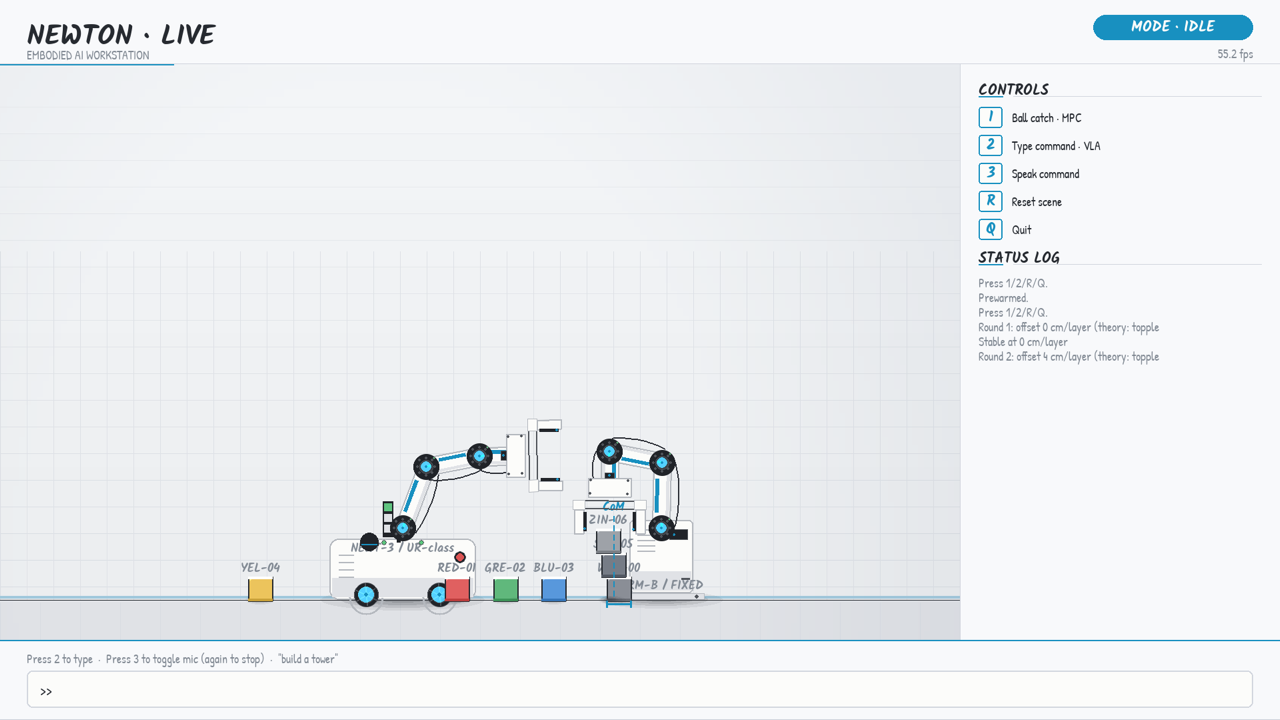
\includegraphics[width=\linewidth]{figures/experiment_offset.png}\\
\footnotesize \textbf{4 cm} · CoM 偏 6 cm $<r$ · \textcolor{green!50!black}{稳}
\column{0.33\linewidth}
\centering
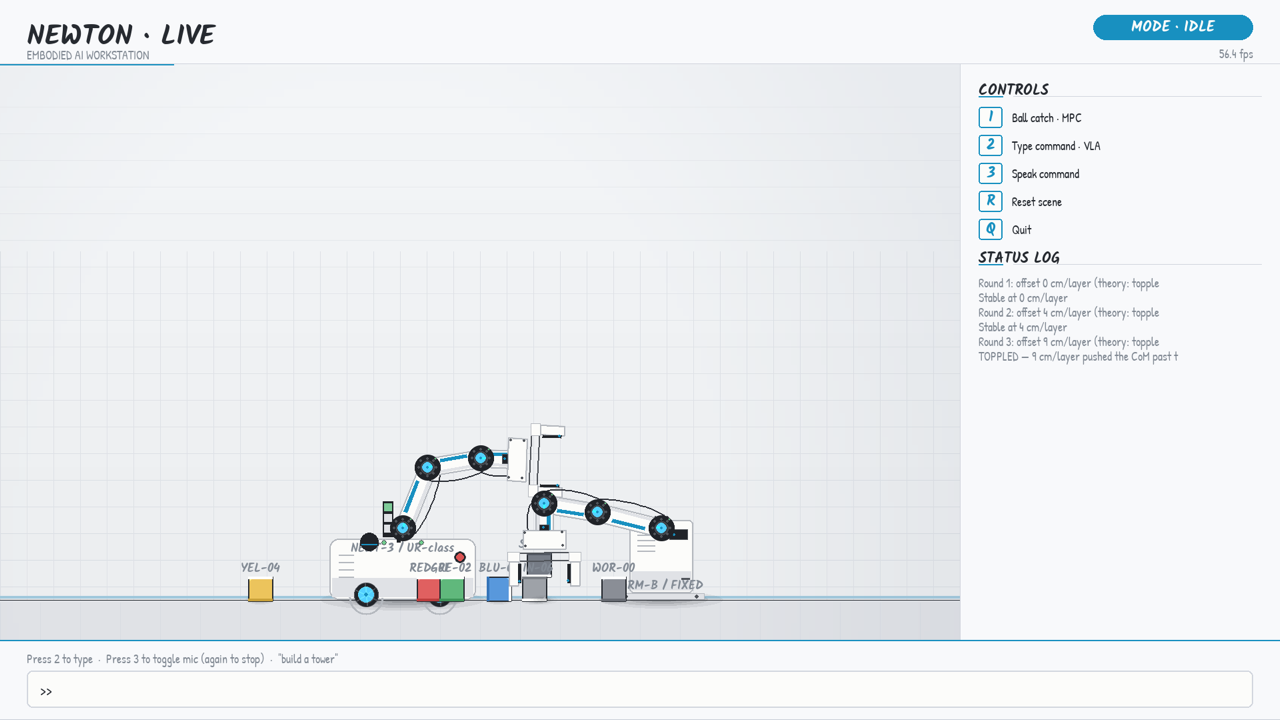
\includegraphics[width=\linewidth]{figures/experiment_topple.png}\\
\footnotesize \textbf{9 cm} · CoM 偏 13.5 cm · \textcolor{red!70!black}{倒}
\end{columns}
\vspace{6pt}
\footnotesize 真求解器回归测试钉死 ``4 cm 稳 / 9 cm 倒'' 的包夹断言——
理论预测与 XPBD 仿真在课堂现场\textbf{逐帧吻合}。
\end{frame}

% ============================================================
\section{视觉反馈设计}

\begin{frame}{戏剧化视觉反馈}
\begin{columns}[T]
\column{0.5\linewidth}
\textbf{接球瞬间}
\footnotesize
\begin{itemize}
\item \textcolor{orange!80!black}{琥珀光环} 标记决策时刻
\item 接到时彩色粒子爆裂
\item 1.5 s 慢动作 (0.33$\times$)
\item 横幅 ``CAUGHT $\cdot$ N''
\end{itemize}

\textbf{命令未识别}
\footnotesize
\begin{itemize}
\item \textcolor{orange!80!black}{琥珀横幅}: ``DIDN'T CATCH THAT''
\item 输入态 footer 自动切到命令示例
\item ``miss'' 音效
\end{itemize}

\column{0.5\linewidth}
\textbf{AI 推理迹侧栏}\\
\scriptsize 7 行实时展开：
\begin{itemize}\scriptsize
\item \texttt{user}: 学生原话
\item \texttt{via}: \texttt{preflight} / \texttt{claude} / \texttt{fallback}
\item \texttt{latency}: 毫秒数
\item \texttt{action}: pick/stack/...
\item \texttt{color} / \texttt{colors}
\item \texttt{target}: [x, z]
\item \texttt{reason}: 自然语言解释
\end{itemize}

\textbf{慢动作 gate}\\
\scriptsize 只在 \texttt{!executor.busy} 时触发，避免
pick/stack 中接球导致动作脱钩。
\end{columns}
\end{frame}

% ============================================================
\section{测试与评估}

\begin{frame}{测试矩阵}
\centering\small
\begin{tabular}{lrl}
\toprule
测试文件 & 测试数 & 重点 \\
\midrule
\texttt{test\_tasks}               & 27 & 程序构造器 + 手势 + 抓取回调 \\
\texttt{test\_vla\_parser}         & 24 & 关键词 (en + zh) \\
\texttt{test\_voice\_fuzzy}        & 21 & 噪声转录用例 (en + zh) \\
\texttt{test\_render\_smoke}       & 21 & 双渲染路径全部 draw\_* \\
\texttt{test\_pipeline}            & 20 & 所有 action 分支 \\
\texttt{test\_effects}             & 19 & 粒子 / 光环 / 横幅生命周期 \\
\texttt{test\_catcher}             & 18 & 弹道反解 + 状态机 \\
\texttt{test\_vla\_subprocess}     & 17 & Claude CLI mock \\
\texttt{test\_control}             & 13 & PD slew + NaN 拒收 \\
\texttt{test\_telemetry} / \texttt{ik} / \texttt{docs\_site} & 10$\times$3 & CSV / IK / \textbf{落地页校验} \\
\texttt{test\_real\_blocks}        & 9  & \textbf{KINEMATIC 抓取 + 堆叠 + OOB} \\
\texttt{test\_experiment}         & 11 & \textbf{倒塌判据 4cm稳/9cm倒 包夹} \\
\texttt{test\_scripted\_constants} & 7  & 彩排数据 \\
\texttt{test\_scripted\_flows}     & 6  & 端到端流程 \\
\texttt{test\_collab}              & 5  & \textbf{双臂接力 build/teardown/loop} \\
\texttt{test\_display\_mode}       & 2  & CLI 解析 \\
\midrule
\textbf{合计 (18 文件)}            & \textbf{250} & 100\% 通过 / $\sim$105 s \\
\bottomrule
\end{tabular}
\end{frame}

% ============================================================
\begin{frame}{FPS 实测 (Apple Silicon, CPU-only, capped@60)}
\centering\small
\begin{tabular}{lrrrr}
\toprule
场景 (18 s headless bench) & min & avg & max & 样本 \\
\midrule
IDLE 工业模式        & 39.1 & \textbf{54.9} & 277.6 &  973 \\
Scripted stack       & 40.4 & \textbf{54.9} & 478.3 &  974 \\
Scripted VLA         & 42.0 & \textbf{53.9} & 319.4 &  963 \\
\texttt{--collab} 双臂接力 & 40.6 & \textbf{54.6} & 308.2 &  970 \\
\texttt{--real-blocks} 真刚体 & 47.7 & \textbf{55.9} & 134.3 & 1005 \\
\texttt{--experiment} 偏移塔 & 40.9 & \textbf{56.5} & 129.5 & 1014 \\
\bottomrule
\end{tabular}

\vspace{8pt}
\footnotesize
\textbf{读法}：avg 被 \texttt{clock.tick(60)} 钉在 $\sim$55（+macOS 调度抖动/热），
\textbf{不是算力瓶颈}——\textcolor{urcyan}{max 277--478} 暴露了真正的余量。
真刚体 / 偏移塔的 max 较低，因为它们要跑真实碰撞管线（见下页）。
\end{frame}

% ----
\begin{frame}{性能优化：把物理从 71\% 帧预算压到 $\sim$2\%}
\textbf{反直觉发现}：原 \texttt{world.step()} 吃掉 \textbf{11.9 ms}（71\% 的 16.7 ms 帧预算），
但 Newton 只模拟 4 个 body。那 12 ms 几乎全是 \textbf{Warp kernel 启动开销}
（substeps $\times$ collide 管线），不是算力。

\vspace{6pt}
\begin{columns}[T]
\column{0.5\linewidth}
\begin{block}{三个杠杆}
\footnotesize
\begin{enumerate}
\item \texttt{iterations 20$\to$8}、\texttt{substeps 4$\to$2}、\texttt{sim\_dt 1/240$\to$1/120}\\
  \scriptsize 约束：\texttt{substeps$\times$sim\_dt = 1/60}
\item teleport 模式复用空 contacts，\textbf{跳过 per-substep collide}（无真实接触时）
\item teleport solver \texttt{iterations 8$\to$2}（无人读它的物理臂位姿）
\end{enumerate}
\end{block}

\column{0.5\linewidth}
\begin{block}{结果}
\footnotesize
\begin{itemize}
\item \texttt{step()}：11.9 ms $\to$ \textbf{0.30 ms}（\textcolor{urcyan}{$\approx$40$\times$}）
\item uncapped 吞吐：64 $\to$ \textbf{279 fps}
\item 60 fps 预算下 \textbf{4$\times$ 余量}
\item 250 测试全绿、渲染臂 \textbf{0 px} 变化
\end{itemize}
\end{block}
\end{columns}

\vspace{2pt}
\footnotesize\textcolor{gray}{性能数据为优化迭代中 cProfile 实测（uncapped headless）；
当前代码即优化后状态（\texttt{substeps=2, sim\_dt=1/120}），其余量由上页 FPS
表 max 列（277--478）独立佐证。}
\vspace{2pt}
\footnotesize\textcolor{gray}{关键洞察：渲染臂由控制器 FK (\texttt{arm\_state\_from\_target}) 驱动，
不读 solver——所以降迭代对画面零影响。\texttt{--real-blocks} 保留完整 collide（堆叠需要接触）。}
\end{frame}

% ============================================================
\begin{frame}{实战演示数据}
\centering\small
\begin{tabular}{lrrl}
\toprule
日期 & catch & VLA & 备注 \\
\midrule
05-21 12:05 & 7/10  & 0 & 首次现场 \\
05-21 12:30 & 8/13  & 1 & Claude 9.4 s 解析 ``pizza tower'' \\
05-21 17:42 & \textbf{14/17} & 0 & 30 s 密集投球 \\
\bottomrule
\end{tabular}

\vspace{18pt}
\begin{block}{典型 telemetry CSV 节选}
\scriptsize\ttfamily
\begin{tabular}{lll}
elapsed & event & detail \\
1.96 & mode & ball\_catch \\
4.48 & catch & 1/2 \\
6.45 & catch & 2/3 \\
\dots & \dots & \dots \\
30.10 & catch & 14/17 \\
\end{tabular}
\end{block}
\end{frame}

% ============================================================
\section{工程教训}

\begin{frame}{工程教训：发现与修复的 bug}
\textbf{第三方专业评审找出 13 个问题，全数闭环}
\vspace{4pt}
\begin{itemize}\footnotesize
\item \textcolor{red!70!black}{\textbf{CRITICAL}} preflight 白名单漏手势 $\to$ 手势必须等 Claude 9.4 s
\item \textcolor{red!70!black}{\textbf{CRITICAL}} point 方向被颜色过滤吃掉 $\to$ 永远退化为 left
\item \textcolor{orange!80!black}{HIGH} slow-mo 在 pick/stack 中触发 $\to$ 动作脱钩
\item \textcolor{orange!80!black}{HIGH} parse\_thread 旧线程结果覆盖新命令
\item \textcolor{orange!80!black}{HIGH} \texttt{test\_scripted\_catch} 抗 flake 不足
\item \textcolor{gray}{MEDIUM} voice \texttt{socket.setdefaulttimeout} 进程级污染
\item \textcolor{gray}{MEDIUM} Arm B 在 rehearsal 里重复 pipeline 逻辑
\item \textcolor{gray}{MEDIUM} CSV \texttt{=cmd} Excel 公式注入
\item \textcolor{gray}{MEDIUM} \texttt{pipeline.build\_plan\_from} 无单测
\item \textcolor{gray}{MEDIUM} \texttt{telemetry} 类型注解不准
\item \textcolor{gray}{LOW} O(n²) \texttt{list.index()} 块越界恢复
\item \textcolor{gray}{LOW} \texttt{launch\_ball} 速度无上限
\item \textcolor{gray}{LOW} 死代码桩 \texttt{\_request\_exit}/\texttt{\_finish}
\end{itemize}

\vspace{4pt}
\textbf{发现的隐藏 bug}：固定臂 \texttt{\_ensure\_reachable} 误驱动主臂底盘。
\end{frame}

% ============================================================
\begin{frame}{代码进化：v0.1.0 $\to$ v0.2.0}
\centering\small
\begin{tabular}{ll}
\toprule
轮次 & 重点 \\
\midrule
A--D & 测试安全网、scene 拆分、表现力、4 新功能 \\
R--S & 13 个评审修复 (2 CRITICAL) + 抛光 \\
T--V & effects/control/catcher/VLA mock 测试 \\
W--Y & Arm B 构造收敛、空闲循环、修固定臂 drive bug \\
\midrule
\multicolumn{2}{l}{\textbf{v0.2.0（提升技术上限）}} \\
性能 & 三杠杆：物理 11.9\,ms $\to$ 0.30\,ms（$\approx$40$\times$） \\
真物理 & \texttt{--real-blocks} KINEMATIC 抓取 + 真实堆叠/倒塌 \\
协作 & \texttt{--collab} 双臂接力搭塔（多智能体编排） \\
物理课 & \texttt{--experiment} 偏移塔倒塌（理论 vs 仿真） \\
落地页 & GitHub Pages + 校验测试 + 设计报告/slides \\
\midrule
合计 & 测试 41 $\to$ \textbf{250}、零回归、上线演示站 \\
\bottomrule
\end{tabular}
\end{frame}

% ============================================================
\section{总结与展望}

\begin{frame}{已完成 vs 局限}
\begin{columns}[T]
\column{0.5\linewidth}
\textbf{已完成 \checkmark}
\footnotesize
\begin{itemize}
\item 三模式交互 (catch / VLA / gesture)
\item 混合 VLA 解析 (preflight + Claude)
\item \textbf{真实刚体物理} (\texttt{--real-blocks})
\item \textbf{双臂协作搭塔} (\texttt{--collab})
\item \textbf{偏移塔物理课} (\texttt{--experiment})
\item \textbf{物理 $\approx$40$\times$ 优化}（11.9$\to$0.30 ms）
\item 250 测试，稳定 60 fps，上线演示站
\end{itemize}

\column{0.5\linewidth}
\textbf{局限 $\bullet$}
\footnotesize
\begin{itemize}
\item \texttt{\_\_main\_\_.py} 1358 行 > 800 上限，需 AppState 重构
\item \texttt{--collab --real-blocks} 跨周期会漂移，演出用 teleport 接力
\item 慢动作是简化版，非逐帧 replay
\item 语音仅 zh-CN / en-US
\item 接球 MPC 单步式无前瞻
\end{itemize}
\end{columns}

\vspace{12pt}
\textbf{未来工作}
\footnotesize
\begin{enumerate}
\item AppState dataclass 重构主循环 $\to$ \texttt{\_\_main\_\_.py} $\leq 200$ 行
\item \texttt{--collab --real-blocks} 跨周期防漂移（释放阻尼 / 投放微调）
\item 完整逐帧 snapshot replay (D.3 原版)
\item 多语言扩展 (日 / 韩 / 西)
\end{enumerate}
\end{frame}

% ============================================================
\begin{frame}{Q\,\&\,A}
\vspace{30pt}
\centering
\Large \textbf{Q\,\&\,A}
\vspace{18pt}

\normalsize
\textcolor{gray}{Demo 入口（规范仓库根 Makefile）：}\\[6pt]
\texttt{make demo}\;/\;\texttt{industrial}\;/\;\texttt{collab}\;/\;\texttt{experiment}\\[12pt]

\textcolor{gray}{测试入口：}\\[6pt]
\texttt{make test}\quad（完整 250 测试，需兄弟 \texttt{../newton}）\\
\texttt{make test-ci}\quad（101 个 no-newton 子集）\\[12pt]

\textcolor{gray}{在线：}\;
\texttt{hollis36.github.io/newton-vla-demo}\\[12pt]

\textcolor{gray}{release：}\quad \texttt{v0.2.0}\quad（GitHub tag + release）
\end{frame}

\end{document}
